\documentclass[11pt]{article}

% Packages
\usepackage{amsmath, amsthm, amssymb}
\usepackage{hyperref}
\usepackage{graphicx}
\usepackage[utf8]{inputenc}
\usepackage{geometry}
\usepackage{enumitem}
\geometry{a4paper, margin=1in}

%\newcommand{\ignore}[1]{}
%\newcommand{\elaine}[1]{{\color{red} [elaine: #1]}}


% Theorem Environments
\newtheorem{theorem}{Theorem}
\newtheorem{remark}{Remark}
\newtheorem{lemma}[theorem]{Lemma}
\newtheorem{corollary}[theorem]{Corollary}
\newtheorem{definition}[theorem]{Definition}
\newtheorem{proposition}[theorem]{Proposition}

\usepackage{enumitem}
\usepackage{mdframed}
\usepackage{subcaption}
\usepackage[capitalize,noabbrev]{cleveref}

\newcommand{\PRF}{\ensuremath{{\sf PRF}}}
\newcommand{\FHE}{\ensuremath{{\sf FHE}}}
\newcommand{\Gen}{\ensuremath{{\sf Gen}}}
\newcommand{\Eval}{\ensuremath{{\sf Eval}}}
\newcommand{\Enc}{\ensuremath{{\sf Enc}}}
\newcommand{\Dec}{\ensuremath{{\sf Dec}}}
\newcommand{\Seed}{\ensuremath{{\sf Seed}}}
\newcommand{\DB}{\ensuremath{{\sf DB}}}
\newcommand{\Comm}{\ensuremath{{\sf Comm}}}
\newcommand{\xor}{\ensuremath{\oplus}}
\newcommand{\Sim}{\ensuremath{{\sf Sim}}}
\newcommand{\negl}{\ensuremath{{\sf negl}}}
\newcommand{\sk}{\ensuremath{{\sf sk}}\xspace}
\newcommand{\pk}{\ensuremath{{\sf pk}}\xspace}
\newcommand{\ignore}[1]{}
\newcommand{\key}{\ensuremath{{\sf key}}}
\newcommand{\getr}{\ensuremath{~{\overset{\$}{\leftarrow}}}~}

\newcommand{\elaine}[1]{{\color{red} [elaine: #1]}}
\newcommand{\mingxun}[1]{{\color{red} [mz: #1]}}

\definecolor{darkgreen}{RGB}{34, 139, 34}
\definecolor{darkred}{rgb}{0.5, 0, 0}
\definecolor{lightblue}{RGB}{0,176,240}


% Document Information
\title{{\Large Cryptography meets algorithms (15893) Lecture Notes}\\[5pt]
{\bf Lecture 12: Oblivious Data Structures}}
\author{Scribe: Tanisha Saxena}
\date{\today}

\usepackage{caption}
\usepackage{subcaption}
\usepackage[capitalize,noabbrev]{cleveref}

\begin{document}

\maketitle

\section{Motivation}
In previous lectures, we learned Oblivious RAM (ORAM),
which allows us to 
compile {\it any} program into an oblivious counterpart. 
However, in practice, when you encounter
a specific computational task, using generic ORAM  
to compile a non-oblivious algorithm may not 
be the best approach. 
%However, this sort of generic application can cause unnecessarily high overhead. 
For example, in a previous lecture, 
we showed how to design oblivious  
sorting algorithms that asymptotically outperform
the na\"ive approach of directly using ORAM
to compile Quick Sort. 
In this lecture, we will how to design
customized oblivious data structures 
(e.g., dictionary, stack, queue, priority queue) 
that outperform 
generically using Path ORAM to compile a non-oblivious algorithm.
%we saw how ORAM could be used on sorting which caused $O(\log n)$ overhead. Instead, we can actually use the non-recursive tree idea from Path ORAM  to create oblivious data structures that allow us to more easily create oblivious protocols with lower overhead \cite{stefanov2018path}.



\section{Background}
Several of our algorithms will rely on a (non-recursive) ORAM tree
 which was used in Path ORAM~\cite{stefanov2018path}.  
Recall that in the ORAM tree, every element is assigned
to some random path (from the root to some leaf node) --- 
we call this path the  
element's {\it position identifier}.
Suppose one already knows which path an element 
is assigned to, then to fetch the element,
the client performs the following:
\begin{itemize}
\item 
read the corresponding path  
and remove the element 
from the path;
\item 
assign the element to a random new path,
and write it back to the root;
\item 
perform an eviction operation 
on the path just read. 
\end{itemize}

We shall assume that the client stores a superlogarithmically sized
stash (which is required for storing the overflowing elements in Path ORAM), 
and we count cost in terms of the number of elements 
communicated 
to and from the server for each data structure request.
%Henceforth
%we shall assume that the Path ORAM's stash is part of the root.
%In other words, the root has super-logarithmic capacity
%whereas all other nodes 
%in the tree has capacity $4$.

In Path ORAM, to find out which path the desired element 
resides on, we recursively store a position map 
in  a smaller ORAM tree. 
The size of the position map is at least a constant factor
smaller than the original ORAM. Therefore, after logarithmically
many recursions, the position map becomes constant in size
and can be stored directly by the ORAM client.



%Recall the recursive tree data structure used in Path ORAM \cite{stefanov2018path}. In this protocol, the client stores a small local stash. The server-side storage is treated as a tree of buckets where each block is stored in a random leaf and the unique path from the root to said leaf contains all the blocks not in the client stash. An access to Path ORAM can be described by the simple pseudocode shown in Figure \ref{fig:pathORAMpseudo}.

\ignore{
\begin{figure}
    \centering
    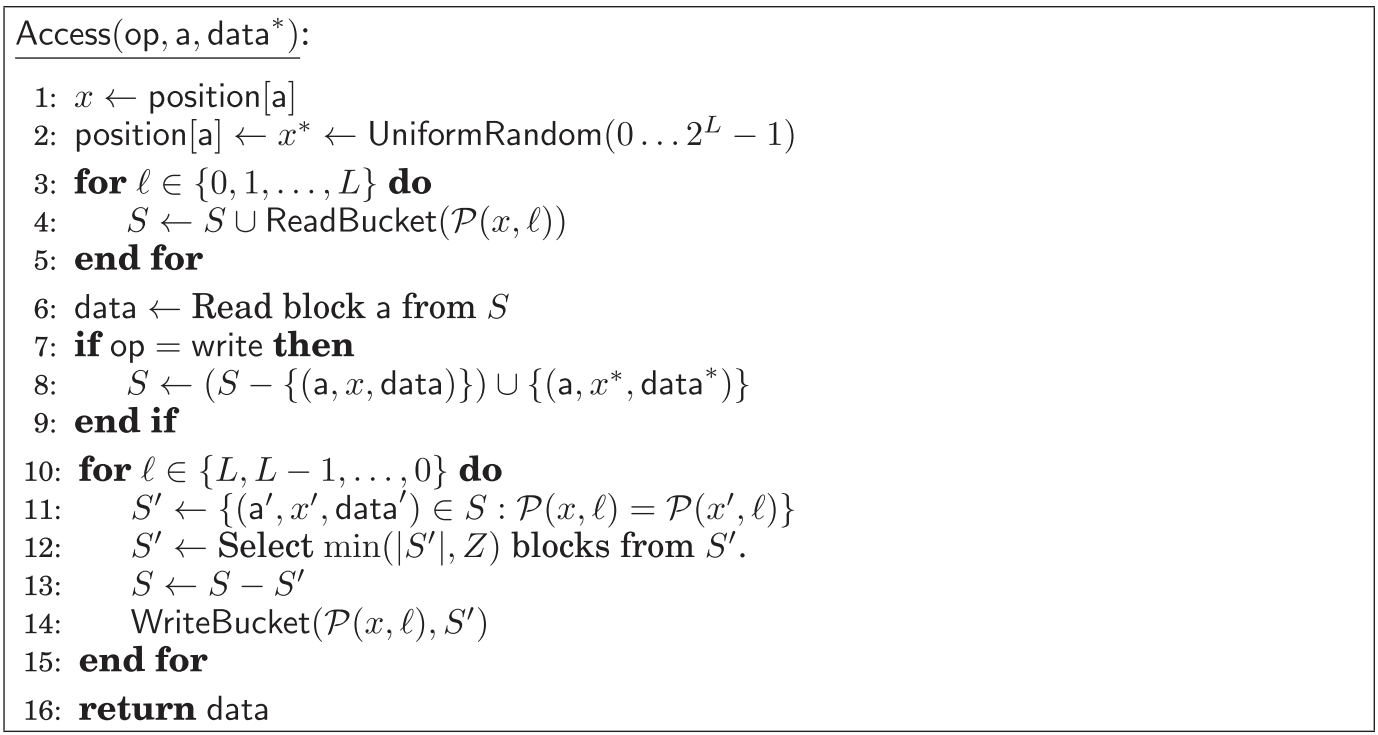
\includegraphics[scale=0.5]{path_oram_pseudocode.png}
    \caption{Pseudocode taken from \cite{stefanov2018path} showing the logic necessary to make an oblivious access in the Path ORAM model}
    \label{fig:pathORAMpseudo}
\end{figure}
}


\section{Oblivious Dictionary}
\subsection{Operations}
%For an oblivious dictionary, we want to support the following operations \cite{wang2014oblivious}:
We consider a standard dictionary data structure
supporting the following operations: 
\begin{itemize}
    \item \textbf{Lookup($k$):} Return the value with key $k$
    \item \textbf{Insert($k, v$):} Insert the value $v$ with key $k$ into the dictionary
    \item \textbf{Delete($k$):} Delete the value with key $k$ from the dictionary
\end{itemize}
Though this oblivious dictionary method can be generalized to include duplicate keys, we will only focus on the case where all keys are unique for the sake of simplicity. Note that ORAM itself 
realizes a memory array abstraction which is 
a special dictionary with contiguous key space $[1\ldots N]$
where $N$ is the maximum number of elements in the data structure.
For a general dictionary, however, the key space is allowed
to be much larger than the number of elements.

%can be viewed as a special case of the dictionary (lookup is a ``read" and insert is a ``write") where the key space is contiguous.

\subsection{Construction for a Static Dictionary}
For simplicity, let's first assume
that we want to implement a static dictionary 
where we only need to support ${\bf Lookup}$ but no dynamic insertion
and deletion. 

The na\"ive approach is to use Path ORAM to directly compile a non-oblivious
dictionary, e.g., an AVL tree --- henceforth we shall
call the AVL tree the {\it logical} tree to distinguish
it from the ORAM tree.
The cost per operation for a non-oblivious AVL tree is $O(\log N)$
where $N$ is the maximum number of elements in the data structure, 
and the Path ORAM
compilation incurs $O(\log^2 N)$ multiplicative overhead.
So the na\"ive approach would incur $O(\log^3 N)$ 
cost per dictionary operation. Note that 
in an AVL tree, not all operations
take the same amount of time. 
When we use ORAM to compile an AVL tree, we have to pad all operations to
the same length to avoid leakage through the number of 
accesses.


%A naive way to implement dictionaries would be to compile a classic logical tree with ORAM. This would involve giving each element a key alongside its value to generate a logical tree as depicted in Figure \ref{fig:bin_tree}. Even if we assume, for simplicity, that the tree is balanced and static, it's still an inefficient way to make an oblivious dictionary. Instead, we can encode a logical tree \textit{within} the recursion used by Path ORAM itself.

\ignore{
\begin{figure}
\centering
\begin{minipage}{.45\textwidth}
  \centering
  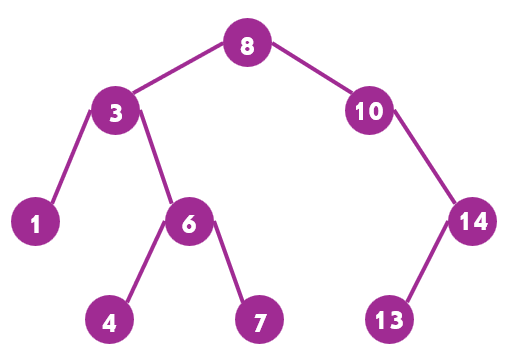
\includegraphics[scale=0.6]{bin_tree.png}
  \captionof{figure}{Naive logical tree compiled with ORAM}
  \label{fig:bin_tree}
\end{minipage}\hfill %
\begin{minipage}{0.45\textwidth}
  \centering
  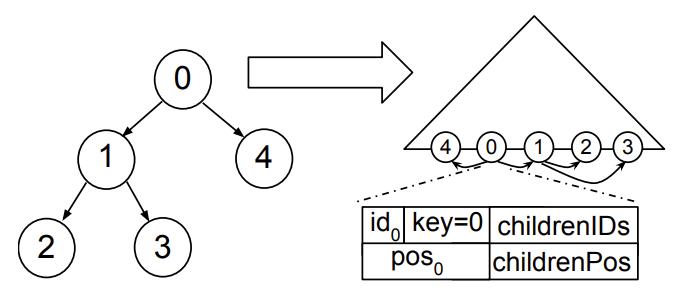
\includegraphics[scale=0.5]{oram_bin_tree.png}
  \captionof{figure}{A diagram representation of a block within the oblivious binary tree \cite{stefanov2018path}}
  \label{fig:oram_bin_tree}
\end{minipage}
\end{figure}
}
\begin{figure*}[t]
\centering
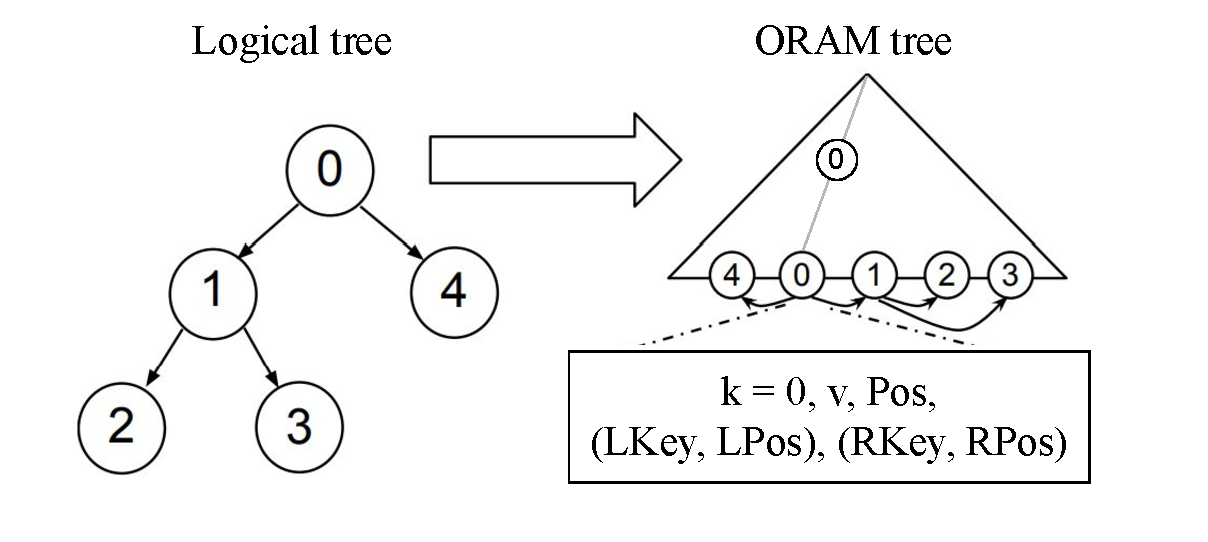
\includegraphics[width=0.8\textwidth]{ods}
\caption{{\bf Each element in the ORAM tree corresponds to a node 
in the logical tree.  
Each element stores
the position identifiers of its two children. 
This eliminates the need to perform a recursive position map lookup
for the next child node to read.}
Note that the element is actually stored somewhere
along the path leading to the leaf even though we draw it at the leaf.
$({\sf LKey}, {\sf LPos})$
and $({\sf RKey}, {\sf RPos})$
denote the 
keys and the position identifiers of the two children.
${\sf Pos}$ denotes the position identifier
of the current element,  
which is needed for performing eviction on the ORAM tree.
}
\label{fig:ods}
\end{figure*}

%\paragraph{Avoiding the recursive position map lookup.}
If we directly use Path ORAM to compile the AVL logical tree, 
essentially we have to go through the entire ORAM recursion for reading
every node in the logical tree. 
The following simple idea~\cite{gentryods,wang2014oblivious} allows
us to avoid this recursion 
overhead. 

As shown in \Cref{fig:ods}, each element in the ORAM tree
corresponds to a node in the logical tree. 
We will have each element 
additionally store the position identifiers of its two children.
Moreover, the client always
stores the position identifier of the logical root.
When the client has fetched some node 
in the logical tree, it immediately knows
the position identifiers of its two children, and hence there is
no more need to do a recursive position map lookup to find
out the next child node it wants to read.


%\elaine{TODO: write a clean version of the algorithm}

More formally, we can implement ${\bf Lookup}(k)$
as follows:
Initially, let $k'$ be the key of 
the logical root, let ${\sf Pos}$ denote
the position identifier of the root.
Let $D = 1.44 \log N$ which corresponds
to the maximum depth of an AVL tree with 
$N$ elements.
Sample $D$ new position identifiers
denoted ${\sf Pos}'_0, \ldots, {\sf Pos}'_D$, and let ${\sf Pos}'_{D+1} = \bot$.
Initialize ${\sf found} := {\sf false}$.
Now, 
for $i = 1$ to $D + 1$, repeat the  
following:
\begin{itemize} 
\item 
If not ${\sf found}$, then 
read and remove the element with key $k'$ from 
 the path ${\sf Pos}$. 
%\begin{itemize}
%\item 
Let $(k', v, {\sf Pos}, ({\sf LKey}, {\sf LPos}), 
({\sf RKey}, {\sf RPos}))$
be the element found:
\begin{itemize}[leftmargin=5mm]
\item 
if $k < k'$, then 
write back
$(k', v, {\color{red} {\sf Pos}'_{i-1}}, ({\sf LKey}, 
{\color{red}{\sf Pos}'_i}), ({\sf RKey}, {\sf RPos}))$
to the root and let $k' := {\sf LKey}$; 
\item 
else 
if $k > k'$, 
write back
$(k', v$, ${\color{red}{\sf Pos}'_{i-1}}$,
 $({\sf LKey}$,
${\sf LPos})$,
$({\sf RKey}$,
${\color{red}{{\sf Pos}'_i}}))$ to the root, and let
$k' := {\sf RKey}$;
\item 
else if $k = k'$, let ${\sf found} := {\sf true}$, 
let ${\sf fetched} := (k', v, {\sf Pos}, ({\sf LKey}, {\sf LPos}), 
({\sf RKey}, {\sf RPos}))$, 
and write back 
$(k', v, {\color{red}{\sf Pos}'_{i-1}}, ({\sf LKey}, {\sf LPos}), 
({\sf RKey}, {\sf RPos}))$
to the root;
\end{itemize}
%\item 
%Else, write back a filler element to the root;
%\item 
%let $i := i + 1$;
%\end{itemize}
\item 
Else if ${\sf found}$, then 
access a random path in the ORAM tree, and write back a filler
element to the root.
\item 
Perform eviction on the ORAM tree path just read.  
\end{itemize}
Finally, the client updates the root's position identifier 
to be ${\sf Pos}'_0$, and the result of the request
is stored in ${\sf fetched}$.

\ignore{
When the client has read 
a path in the logical tree
containing logarithmically many nodes, 
it can choose 
random new position identifiers for all logical nodes 
along this path. 
It then updates the entries 
to make sure that 
each parent correctly points to the new position identifers
for its children, before writing them back to the root
and performing evictions on the ORAM tree.

}

\begin{remark}
In a non-oblivious AVL tree, the lookup algorithm 
stops whenever the desired key is found.
However, in an oblivious dictionary, such early stopping
would leak information 
about where the 
requested element
is in the logical tree. 
Therefore, even after we have found
the element, we still have to perform fake
operations on the ORAM tree, such that all requests 
incur the same number of memory accesses.
%It is known that the maximum height of an AVL
%tree with $N$ elements is $1.44 \log N$.
%Therefore, when the 
%lookup on the logical tree has ended, we will still
%access some more random paths in the ORAM tree, such that 
%the total number of paths accessed is exactly $1.44 \log N$.
\end{remark}

%\subsection{Performance}
\paragraph{Performance.}
The above algorithm involves visiting
$O(\log N)$ ORAM tree paths for each lookup request. 
Therefore, the cost per ${\bf Lookup}$ is $O(\log^2 N)$.


%The improved oblivious data structure has an overhead of $O(\log^2 n)$ with $O(\log n)$ from the recursion level and $O(\log n)$ from the size of the tree. This is an improvement in contrast to the naive approach that compiles binary searching--which automatically incurs a $O(\log n)$ search cost \cite{gentry2013optimizing}-- with Path ORAM--that already has a $O(\log^2 n)$ lookup cost-- giving an overall $O(\log^3 n)$ overhead.

%It is possible to achieve $O(\log n)$ overhead as shown by Asharov et. al. \cite{asharov2023futorama}. With this low overhead, this implementation of an oblivious dictionary finally becomes practical and a viable choice for real-world security. However, there are many restrictions and assumptions that must be met before FuturORAMa can be used and thus some people still prefer to use Path ORAM or Circuit ORAM despite the larger overhead.


%Further, the client records the new position identifier
%for the root node. 


\paragraph{Extending it to a dynamic dictionary.}
The above idea was first suggested by Gentry et al.~\cite{gentryods}
who considered a static logical tree that supports
only ${\bf Lookup}$ but no dynamic insertion and deletion.  
Subsequently, Wang et al.~\cite{wang2014oblivious}
showed that it is not hard to extend the idea to support dynamic 
insertions and deletions.
Specifically, during an insertion or deletion operation, 
the logical AVL tree may perform rotation operations
to balance the logical tree.
Each rotation operation involves modifying the pointers
on constant number of nodes 
in the logical AVL tree. 
In our case, during a rotation, 
we just have to additionally
update the children position identifiers
for nodes involved in the rotation. 
Again, we have to pad all 
requests to the same length 
to avoid leakage through early stopping. 


\ignore{
The implementation of a dictionary with binary search trees is simple and intuitive. Each block can be described as containing the following: a key, a value, a pointer to the current block's path, the left key, a pointer to the left child's path, the right key, and a pointer to the right child's path as can be seen in Figure \ref{fig:oram_bin_tree}.
}


\ignore{
\subsection{Access Protocol}
The only part of the access protocol that differs significantly from the regular setup of Path ORAM is the existence of parents and children. Thus, we must simply maintain the invariant that the parent's child pointers get updated whenever the child's own path is changed on access. This idea can be extended for insertion and deletion in dynamic trees but it remains within the same complexity class for overhead. Beyond that, the access protocol is very similar to the pseudocode shown in Figure \ref{fig:pathORAMpseudo}.
}


\begin{remark}
Using an optimal ORAM like OptORAMa~\cite{optorama} 
to directly compile an AVL tree also gives $O(\log^2 N)$
cost per operation. 
However, the resulting scheme is less practical and has only computational
security, since the only known optimal ORAM constructions
%are based on the hierarchical ORAM framework, 
all rely on the existence of a pseudorandom function.
The aforementioned constructions that makes non-blackbox usage of  
Path ORAM~\cite{stefanov2018path}
or Circuit ORAM~\cite{circuitoram}'s non-recursive ORAM tree 
are conceptually simpler, more efficient in hardware enclave
or secure computation scenarios, and 
enjoy statistical security.
\end{remark}


\section{Oblivious Stacks / Queues}
An oblivious stack or queue can also be realized
using a similar idea.
For example, in an oblivious stack,
each element can store the position identifier
of the next element, and the client saves
the position identifier of the top of the stack denoted ${\sf Pos}_0$.
For a push operation, the client 
%creates a new element assigned to a random path ${\sf Pos}^*$,
assigns the new element to a random path ${\sf Pos}^*$, 
and the have the new element record
${\sf Pos}_0$ as the next element's position identifier. 
The client now writes the new element to the root bucket,
and performs eviction on a random path.
The client also updates ${\sf Pos}_0 := {\sf Pos}^*$.
A pop operation can be implemented in a similar manner.
In this 
way, 
each push or pop operation involves
accessing only a single path in the ORAM tree,
and the cost is $O(\log N)$.


A queue can also be realized in a similar
manner, incurring $O(\log N)$ cost per ${\sf PushBack}$ or
${\sf PopFront}$ operation.

\ignore{
\subsection{Operations}
Zahur et. al. also proposes a circuit-based construction of a stack/queue but, for the proof of concept, we will only describe the Path ORAM implementation for stacks \cite{zahur2016revisiting}. Note that oblivious queues can be made in a very similar way. The oblivious stack supports the following operations \cite{toft2011secure}:
\begin{itemize}
    \item \textbf{Push($v$):} Push the value $v$ on the stack
    \item \textbf{Pop():} Pop the top element off the stack and return it
\end{itemize}

\subsection{Construction}
You only need one tree to store a stack. Then, the head pointer holds the path on which the head of the stack resides. Each item holds a value, $v$, a pointer to itself, and a pointer to the next block's path.

\subsection{Access Protocol}
Push simply requires us to choose a path for the new element and then put it onto the stack by setting it to the new head. Pop is very similar and just pops off and removes the current head of the stack.

\subsection{Overhead}
Because there is only one tree and we only need to worry about modifying one element in the tree at a time, each operation takes $O(\log n)$ time. Note that this is a randomized algorithm because there is only one tree and thus this scheme uses non-recursive Path ORAM. We'll learn about a deterministic oblivious algorithm in a later section on oblivious Turing machines.
}

\section{Oblivious Priority Queues}
%This oblivious data structure constructed using non-recursive Path ORAM is somewhat similar to that of oblivious stacks and queues but has a few notable differences. For simplicity, we are again assuming that all keys are distinct.

We consider a basic priority queue with only the following
two types of opearations: 

\begin{itemize}
    \item \textbf{${\sf ExtractMin}()$:} Return the item with the minimum key;
    \item \textbf{${\sf Insert}(k, v)$:} Insert the value $v$ with key $k$.
\end{itemize}
For simplicity, we shall assume that all items have distinct
keys, although it is not hard to extend
the algorithm
to support possibly 
duplicate keys.


\subsection{Construction}
%Using the hierarchical ORAM proposed by Kasper and Larsen, we can store the elements in order with a block containing the the value, a self-referential pointer, a pointer to this subtree minimum's path, and the subtree's minimum itself \cite{larsen2018yes} \cite{asharov2023futorama}. \cite{wang2014oblivious}.
We will describe Shi's construction of an oblivious  
priority queue~\cite{shi-opq}, also based on a non-recursive
Path ORAM data structure.


\subsection{Access Protocol}

\subsubsection{Extract-min()}
In extract-min(), we first get the minimum value of this tree, aka the subtree minimum at the root. Let $ptr^*$ denote the path the subtree minimum value resides on. We want to remove the subtree minimum value's record from the path stored in $ptr^*$. To do this, we evict on the path $ptr^*$ and, to maintain correctness, we recalculate the subtree minimum values stored in each node along $ptr^*$'s path. Intuitively, since we're removing the subtree minimum from the path, the subtree minimum of all blocks along that path can change. Note that the subtree minimum of a parent is equal to the minimum between the subtree minimums of its two children, so as long as we update from the leaf node upwards, it only requires $O(\log n)$ overhead.


\subsubsection{Insert(k, v)}
First, we choose a path at random and assign that to the block we want to insert. Then, we add our new block to the root of the tree. Lastly, we perform an eviction on two random paths and recalculate the subtree minimum for each node on the two evicted paths to maintain the correctness property. To maintain the oblivious property, we simply pad either operation such that both operations read the same number of paths. This makes the operations indistinguishable from each other to an outside perspective.

\subsubsection{Other operations}
We can also implement ``$delete(ref)$" where $ref$ is a reference to the pointer we want to delete, and ``$decrease\_key(ref, k')$" where we decrease the key of the value ref is referencing to $k'$. In both these cases, we use references to access the path and ensure that correctness is maintained over the tree.
\begin{itemize}
    \item \textbf{Delete(ref):} Access the path pointer denoted by $ref$, removes the item with key $k$, evicts along the path pointed to by $ref$, and recalculates the subtree minimum for each node along the path
    \item \textbf{Decrease-key(ref, k):} Delete(ref), insert($k', v$)
\end{itemize}

\subsection{Overhead}
As expected, since insertion and extract-min() only require us to update the path the element resides on in linear time, they only incur a $O(\log n)$ overhead.

\section{Oblivious Turing Machines}
\subsection{Operations}
As a reminder, in the oblivious Turing machine model we want to hide whether the Turning machine is going left, right, or staying still on the tape.

\subsection{Construction}
Each level of the structure consists of three ``superblocks" increasing exponentially in size by a power of two (ex: the first level has three superblocks of size 1, the second has three superblocks of size 2, the $i$th level has three superblocks of size $2^i$, and so on) as seen in Figure \ref{fig:turing_blocks}. We denote $HEAD$ to be the head pointer of the Turing machine. We then maintain the following invariant throughout the protocol: When a level is rebuilt--for all except the last $n$th level--HEAD lies in the middle superblock.

\begin{figure}
    \centering
    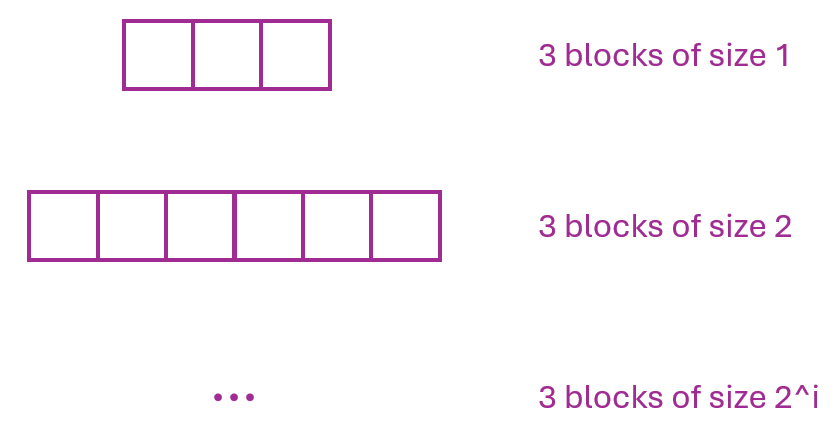
\includegraphics[scale=0.8]{blocks.png}
    \caption{A diagram representation of the levels within an oblivious Turing machine}
    \label{fig:turing_blocks}
\end{figure}

We also want an invariant that indicates how, if level $i$ is updated, all levels $1$ to $(i-1)$ should be notified that $i$ has been updated. The reason for that is each element has multiple copies across levels, thus we must ensure that each copy is updated when the element is updated. This propagation can be done in linear time with respect to the level size.

\subsection{Access Protocol}
The access protocols are easy to implement because a Turing machine can only ``read" or ``write" which can be done with the same access protocol as ORAM as shown in Figure \ref{fig:pathORAMpseudo}.

\subsection{Overhead}
The $i$th level is rebuilt every $2^i$ steps with a rebuilding cost in $O(2^i)$. Thus, over the protocol the costs to rebuild are:
\begin{align*}
    &\textbf{Level 0: } c \cdot 2^0 = c \\
    &\textbf{Level 1: } c \cdot 2^1\cdot \text{ rebuild every 2 steps} \Rightarrow c \cdot 2^0 \text{(amortized)} \tag{Rebuild cost is linear}\\
    &\text{etc } \dots
\end{align*}
At each level we get $c$ work and thus we incur $O(\log n)$ cost per operation. This result is actually quite old and has been proven since Fischer and Pippenger in 1979 \cite{pippenger1979relations}.

\newpage
\bibliographystyle{alpha}
\bibliography{refs.bib}
\end{document}
